\section{Methods} \label{sec:methods}

In this section, we describe the primary two algorithmic components for our on-device simulation: the memory- and compute-efficient genetic design used to annotate genome material to facilitate robust post-hoc phylogenetic reconstruction, and the compute-communicate cycle used to instantiate an evolutionary process with the genetic architecture across the WSE engine.

\subsection{Asynchronous Island-model Evolutionary Computaiton}

We apply an island-model genetic algorithm, which is a commonly used approach to doing evolutionary computation in parallel and distributed computing \citep{kozaTODO}.
In this scheme, each processor elemement (PE) has an independent population.
Migration between PEs links the populations into a network of a single population.
To minimize synchronization costs, we adopt a fully asynchronous approach to migration between neighboring PEs.
Evolutionary processes tend to occur in asynchronous manner with arbitrary factors influencing things, so this is a reasonable relaxation to make.

\begin{wrapfigure}{r}{0.5\textwidth}
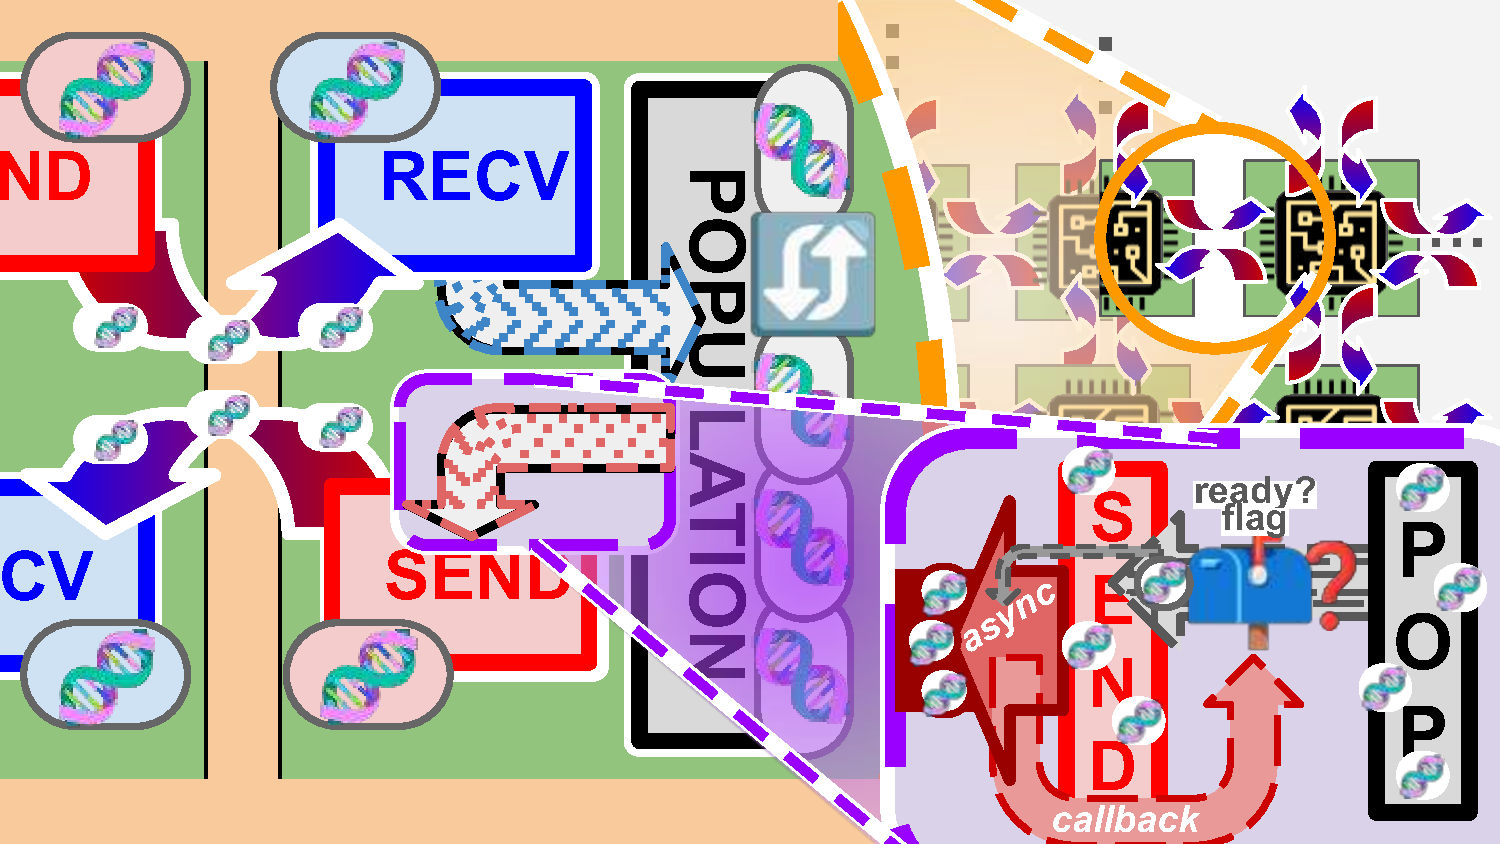
\includegraphics[width=\linewidth]{img/async-ga-schematic.pdf}
\centering
\caption{Schematic overview of asynchronous island model evolutionary algorithm.}
\label{fig:async-ga-schematic}
\end{wrapfigure}


In the core of the algorithm, each PE performs an update cycle, which comprises several steps.
Figure \ref{fig:async-ga-schematic} provides a schematic overview.

The first step of this update loopis to handle migration.
Each PE has an immigration buffer and an emigration buffer for each cardinal neighbor.
On simulation startup, an asynchronous receive request is opened to accept genomes from the neighbor into the immigration buffer.
The emigration buffer is populated with individuals from the population and an asynchronous send request is opened to dispatch wavelets containing genome data from the emigration buffer to the neighbor.
For both operations, a callback is registered to set the send complete or receive complete flag variable for that cardinal direction once the asynchronous operation is satisfied.
Each update cycle, the flags are tested for.
If they are set, then genomes from the transfer buffers are sampled from and/or mixed into the main population, as appropriate for the detected flag, set flags are reset, and new send and/or receive requests are registered.

The remainder of the update loop handles evolutionary operations witin the scope of the executing PE.
Each genome within the population is evaluated to produce a floating point fitness value based on a user-defined criteria.
For the purposes of the work in this project, we will use a trivial fitness function that explicitly models additive accumulation of beneficial/deleterious mutations.
Then, tournament selection is applied.
For each slot in the next generaiton is filled with the highest of $n$ sampled values, with ties broken randomly.
A swap buffer is used to collect individuals for the next generation.
A mutational operator is applied across all genomes in the next population, then the process repeats.
A self-activating wavelet is dispatched to execute the next cycle of the loop.

The source code for this kernel can be viewed at \url{https://hopth.ru/cl}.
Importantly, the implementation is defined modularly with respect to genome size, layout, and fitness evaluation criteria.
This will allow us to readily adjust the particulars of simulation as needed for each project component.

\subsection{Distributed Phylogenetic Tracking}

In pilot work with dynamically curated space-time memory buffers, we have achieved highly-scalable phylogenetic tracking in ABMS modelling of evolutionary processes \citep{morenoHstratPythonPackage2022, morenoHereditaryStratigraphyGenome2022}.
Our approach, hereditary stratigraphy (HStrat), uses a reconstruction-based strategy akin to how biologists build phylogenies.
Using heritable generational fingerprints, we achieve fast, accurate reconstruction.
To prevent $\mathcal{O}(n)$ space complexity, not all fingerprints can be kept.
Instead, we use a constant-time indexing scheme to map a stream of fingerprints onto a fixed-width memory buffer such that entries evicted by new placements maintain a temporally-representative sampling over elapsed time, either evenly (``steady'') or recency-biased (``tilted'') (Fig. \ref{fig:hstrat-schematic}).
Time stamps can be positionally inferred  --- a several-fold savings for small data objects. For example, single-bit checkpoints produce good quality phylogenies using only 12 bytes per genome \citep{moreno2023toward}.

It is necessary to optimize reconstruction to get high quality results with tractable genome sizes and limit the impact on memory usage and bandwidth usage.
Hereditary stratigraphy \citep{moreno2022hereditary} was designed to do this.

We have successfully demonstrated aspects of this approach (published in existing work as the hstrat Python library), with present work revising the underlying algorithms to better suit resource-constrained environments such as CS-2 Processor Elements.
Existing work targets traditional HPC environments \citep{moreno2022hstrat},
However, a highly compact, without advanced data structures is necessary to support the Cerebras WSE.
This led to development of unpublished variant of existing hereditary stratigraphy, the hereditary stratigraphic surface.

\begin{figure}[htbp]
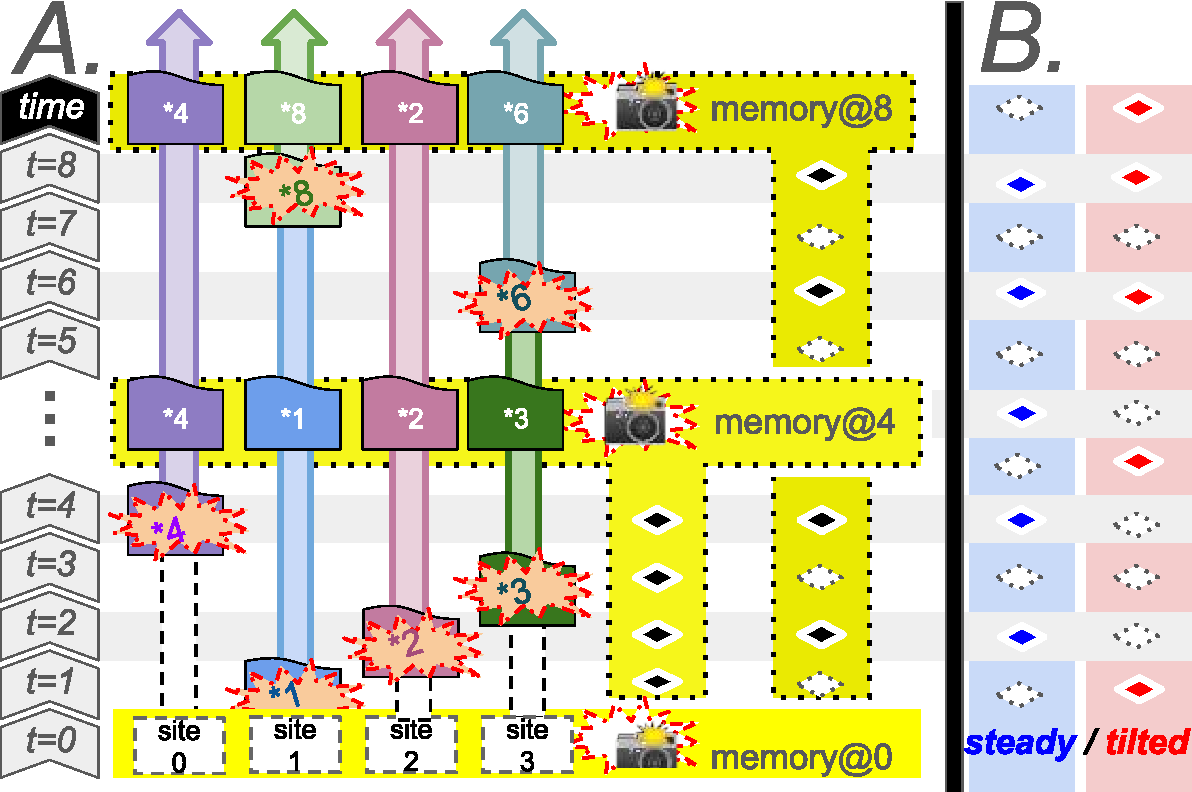
\includegraphics[width=4in]{img/hsurf-schematic.pdf}
\caption{Panel A shows update sequence on a four-site HStrat curation space-time memory under steady policy. Panel B contrasts steady policy with tilted policy, which prioritizes recent data. }
\label{fig:hsurf-schematic}
\end{figure}

Instead of being maintained within a sorted list, lineage checkpoint markers are stored in a flat buffer.
This couples curation --- adding a checkpoint implicitly removes the checkpoint it overwrites.
The indexing scheme can be computed in $\mathcal{O(1)}$ time with respect to the size of the buffer and to the number of generaitons elapsed.

This genome has two components: a generation counter and the checkpoint marker buffer.
